\documentclass[main.tex]{subfiles}

\begin{document}
\KOMAoptions{twoside=false}
\begin{fullsizetitle}
    \vspace{2cm}
    \hspace{0.1\textwidth}
    \vline\hspace{10pt}
    \begin{minipage}[t][0.8\textheight][t]{0.8\textwidth}
        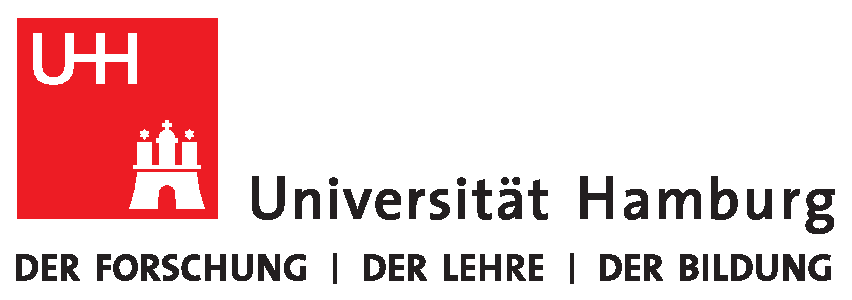
\includegraphics[width=5cm, valign=c]{images/logos/up-uhh-logo-u-2010-u-farbe-u-cmyk}
        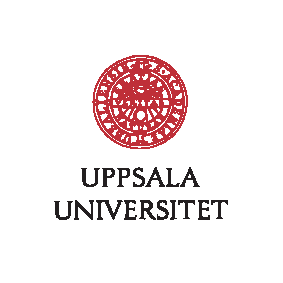
\includegraphics[width=4cm, valign=c]{images/logos/UU_logo_CMYK}\par
        \vspace{1\baselineskip}

    \begin{FlushLeft}
        {\Large\textcolor{UHHred}{Master thesis}\par}

        {\huge Superconducting phase stiffness and coherence length from a finite momentum pairing constraint\par}

       \vspace{1\baselineskip}
       
       May 2025

        %\vspace{4\baselineskip}
    \end{FlushLeft}

    \vfill
    
    \begin{FlushLeft}
    	Tjark Sievers (7147558)\par
        Department of Physics\par
        First reviewer: Prof.\,Dr.\,Annica Black-Schaffer (Uppsala University) \par
        Second reviewer: Prof.\,Dr.\,Tim Wehling \par
    \end{FlushLeft}
    \end{minipage}
\end{fullsizetitle}
\KOMAoptions{twoside=true}

\thispagestyle{plain}

\epigraph{Even Einstein [...] had attempted to construct a theory of superconductivity. Fortunately, I was unaware of these many unsuccessful attempts. So when John invited me to join him (he, somehow, neglected to mention these previous efforts), I decided to take the plunge.}{Leon Cooper \par \enquote{Remembrance of Superconductivity Past}, BCS: 50 Years \cite{cooperBCS50Years2010}.}

\vspace*\fill

\bigskip

\noindent
Typeset with {\LaTeX} in TeX Gyre Pagella, \textsf{TeX Gyre Heros}, and \texttt{TeX Gyre Cursor}.


\end{document}
